%--------------------------------------------------%
%  KAPITOLA 01 - PŘEHLED SOUČASNÉHO STAVU POZNÁNÍ  %
%--------------------------------------------------%

\chapter{PŘEHLED SOUČASNÉHO STAVU POZNÁNÍ}
Tato kapitola se v úvodní části věnuje krátkému představení systému \TeX\ a jeho nadstavbě \LaTeX, v další části je poté sestaven přehled nejpoužívanějších \LaTeX\ editorů, a to jak online, tak i offline/desktopových aplikací.

\section{Systémy \TeX\ a \LaTeX}
Pro formátování vstupního textu slouží formátovací programy. Mezi ně se řadí i \TeX, který byl vytvořen Donaldem E. Knuthem. Účelem bylo vytvořit program pro vysoce profesionální a kvalitní sazbu dokumentů z matematického a technického prostředí. \TeX\ však umožňuje pouze primitivní operace pro sázení dokumentů, které jsou řízeny sadou jednoduchých příkazů, tzv. primitivů. \cite{Kopka}

Primitivy umožňují definovat tzv. makra, tedy složitější a komplexnější příkazy. Tato možnost byla využita Leslie Lamportem, který naprogramoval sadu maker. Vzniklá sada dostala název \LaTeX\ a dnes je nejrozšířenější nadstavbou základního jazyka \TeX. Lamportem naprogramovaná makra umožňují členit dokumenty na kapitoly, přidávat citace, využívat výhod automatického číslování rovnic, používat křížové odkazy nebo jedním příkazem generovat obsah celého dokumentu. Vznikl tak nástroj umožňující užívání celého systému i bez znalostí programování. \cite{Kopka}

Pomocí vytvořených příkazů uživatelé zadávají, co chtějí vysázet. Informace o tom, jak se má zadaný textový řetězec vysázet (velikost písma, odsazení, umístění na straně a další), jsou obsaženy v použitém příkazu. Uživatel díky tomu nepotřebuje typografické znalosti, protože systém \LaTeX\ za něj všechny vstupní textové řetězce vysází sám. \cite{Rybicka}

Systém \LaTeX\ rovněž umožňuje importování balíčků (sad dalších maker), které rozšiřují základní funkcionality o další prvky. Díky tomu se celý systém rozšířil i do oblastí, pro které nebyl zamýšlen. \cite{Kopka}

\begin{figure}[h]
	\centering
	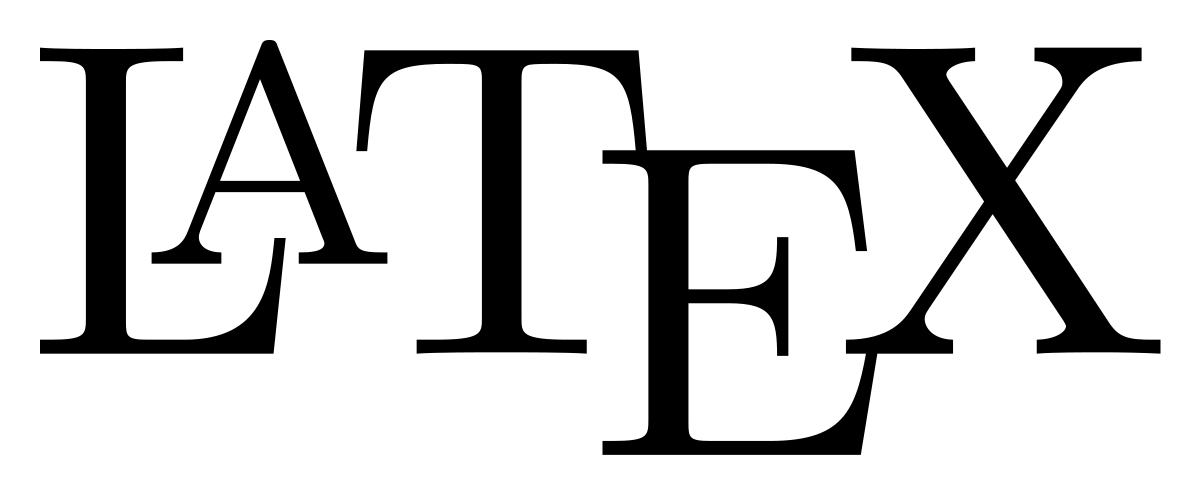
\includegraphics[width=8cm]{obrazky/latex.png}
	\caption[Logo systému \LaTeX.]{Logo systému \LaTeX. [vlastní]}
	\label{fig:latexlogo}
\end{figure}

\TeX\ a \LaTeX\ jsou rovněž nazývány programovacími jazyky. Jejich užití není limitováno žádnými jinými programy, aplikacemi nebo operačními systémy. Pro překlad vstupního textového dokumentu uživatel potřebuje pouze nainstalovanou \LaTeX\ distribuci a libovolný program s překladačem jazyka \TeX. \cite{Kopka}

\section{Přehled \LaTeX\ editorů}
\label{sec:prehled}
Pro tvorbu \LaTeX\ dokumentů existují editory, které uživatelům usnadňují práci. Tyto editory nabízejí barevné rozlišení příkazů pro snadnější orientaci v textu, našeptávání jednotlivých příkazů, možnost úpravy vizuálního vzhledu editoru a další funkcionality. Společným základech všech editorů je integrovaný překladač jazyka \TeX, který ze zdrojového kódu (textový soubor s příkazy a vlastním textovým obsahem) vytvoří požadovaný dokument, například ve formátu PDF. \LaTeX\ dokument lze napsat také v obyčejném poznámkovém bloku, uživatel v něm ale nemá možnost text dále jakkoliv efektivně zpracovat.

Na následujících řádcích byl vytvořen přehled nejpoužívanějších \LaTeX\ editorů s jejich popisem, ukázkou a přehledem výhod a nevýhod. Tento přehled vychází z několika webových příspěvků věnujících se sestavením žebříčku \LaTeX\ editorů \cite{Techpout}\cite{Guru99}\cite{Beebom}.

\subsection{\TeX maker}
\TeX maker editor vznikl v roce 2003 a dnes se řadí k nejoblíbenějším a nejpoužívanějším \LaTeX\ desktopovým editorům. Nabízí přehledné prostředí s podporou českého jazyka, integrovaný PDF prohlížeč tvořeného dokumentu a dnes velmi oblíbený dark-mode uživatelského prostředí. Český jazyk je integrován i na úrovni kontroly pravopisu v reálném čase, tj. během psaní textu. \cite{texmaker}

\begin{figure}[h]
	\centering
	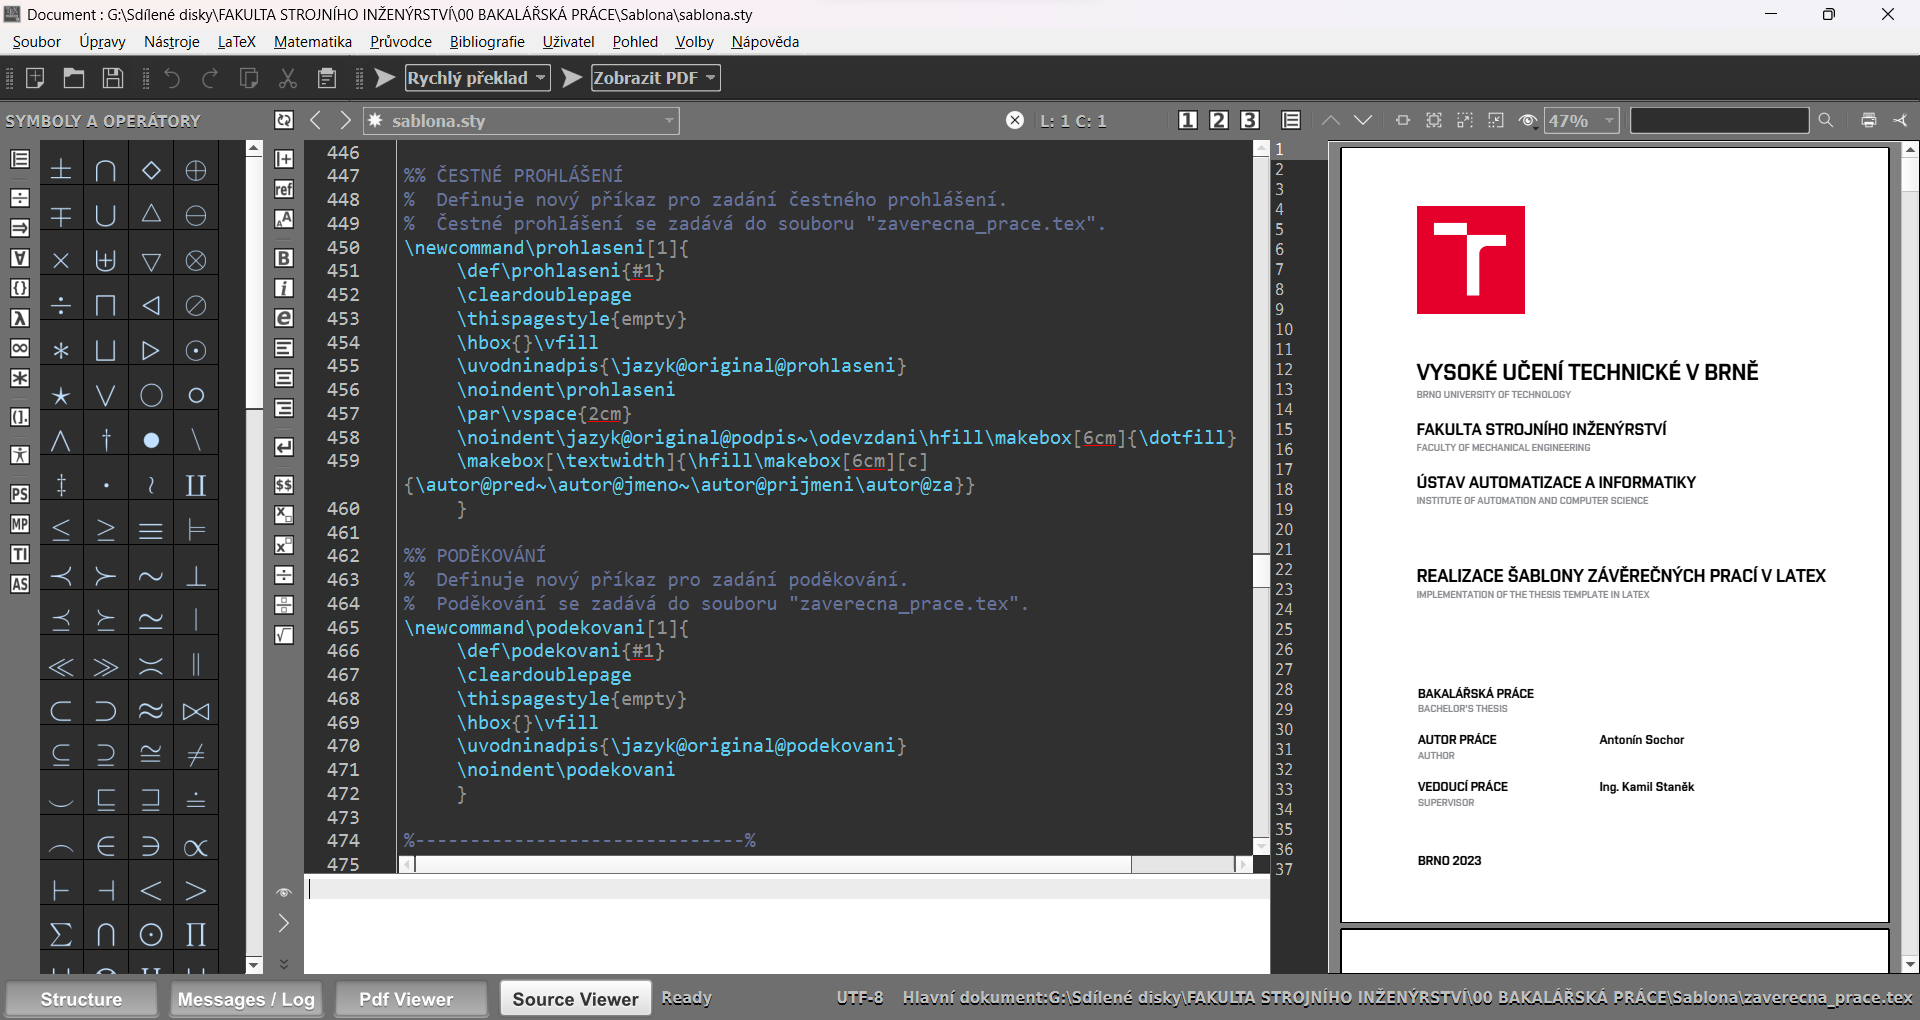
\includegraphics[width=\textwidth]{obrazky/texmaker.png}
	\caption[Ukázka prostředí \TeX maker editoru.]{Ukázka prostředí \TeX maker editoru. [vlastní]}
	\label{fig:texmaker}
\end{figure}

Autoři poskytují řešení pro operační systémy Windows, macOS a Linux. Pro 370 nejpoužívanějších matematických symbolů má \TeX maker samostatná tlačítka, díky kterým není nutné znát jednotlivé příkazy na požadované matematické symboly. Při výskytu chyb editor uživatele upozorní a zobrazí čísla řádků, na kterých se daná chyba nachází. Velkou výhodou je našeptávání základních \LaTeX\ příkazů. Do editoru je integrováno několik překladačů, mezi nimiž může uživatel volně přepínat. Na výběr je \LaTeX, pdf \LaTeX, \LaTeX mk, Xe\LaTeX\ a Lua\LaTeX. \cite{texmaker}

\textbf{Výhody a nevýhody:}
\begin{multicols}{2}
	\begin{itemize}
		\item [+] použití zdarma
		\item [+] uživatelské prostředí v českém jazyce
		\item [+] kontrola pravopisu
		\item [+] verze pro Windows, macOS i Linux
		\item [+] tlačítka pro matematické symboly
		\item [+] našeptávání příkazů
		\item [+] volba překladače zdrojového kódu
		\item [+] integrovaný PDF prohlížeč
	\columnbreak
		\item [--] chybějící překlad některých tlačítek
		\item [--] nevyužívá cloud
	\end{itemize}
\end{multicols}

\subsection{\TeX studio}
Cílem \TeX studio editoru je udělat \LaTeX\ tvorbu co nejjednodušší a nejpohodlnější \cite{Texstudio}.

\begin{figure}[h]
	\centering
	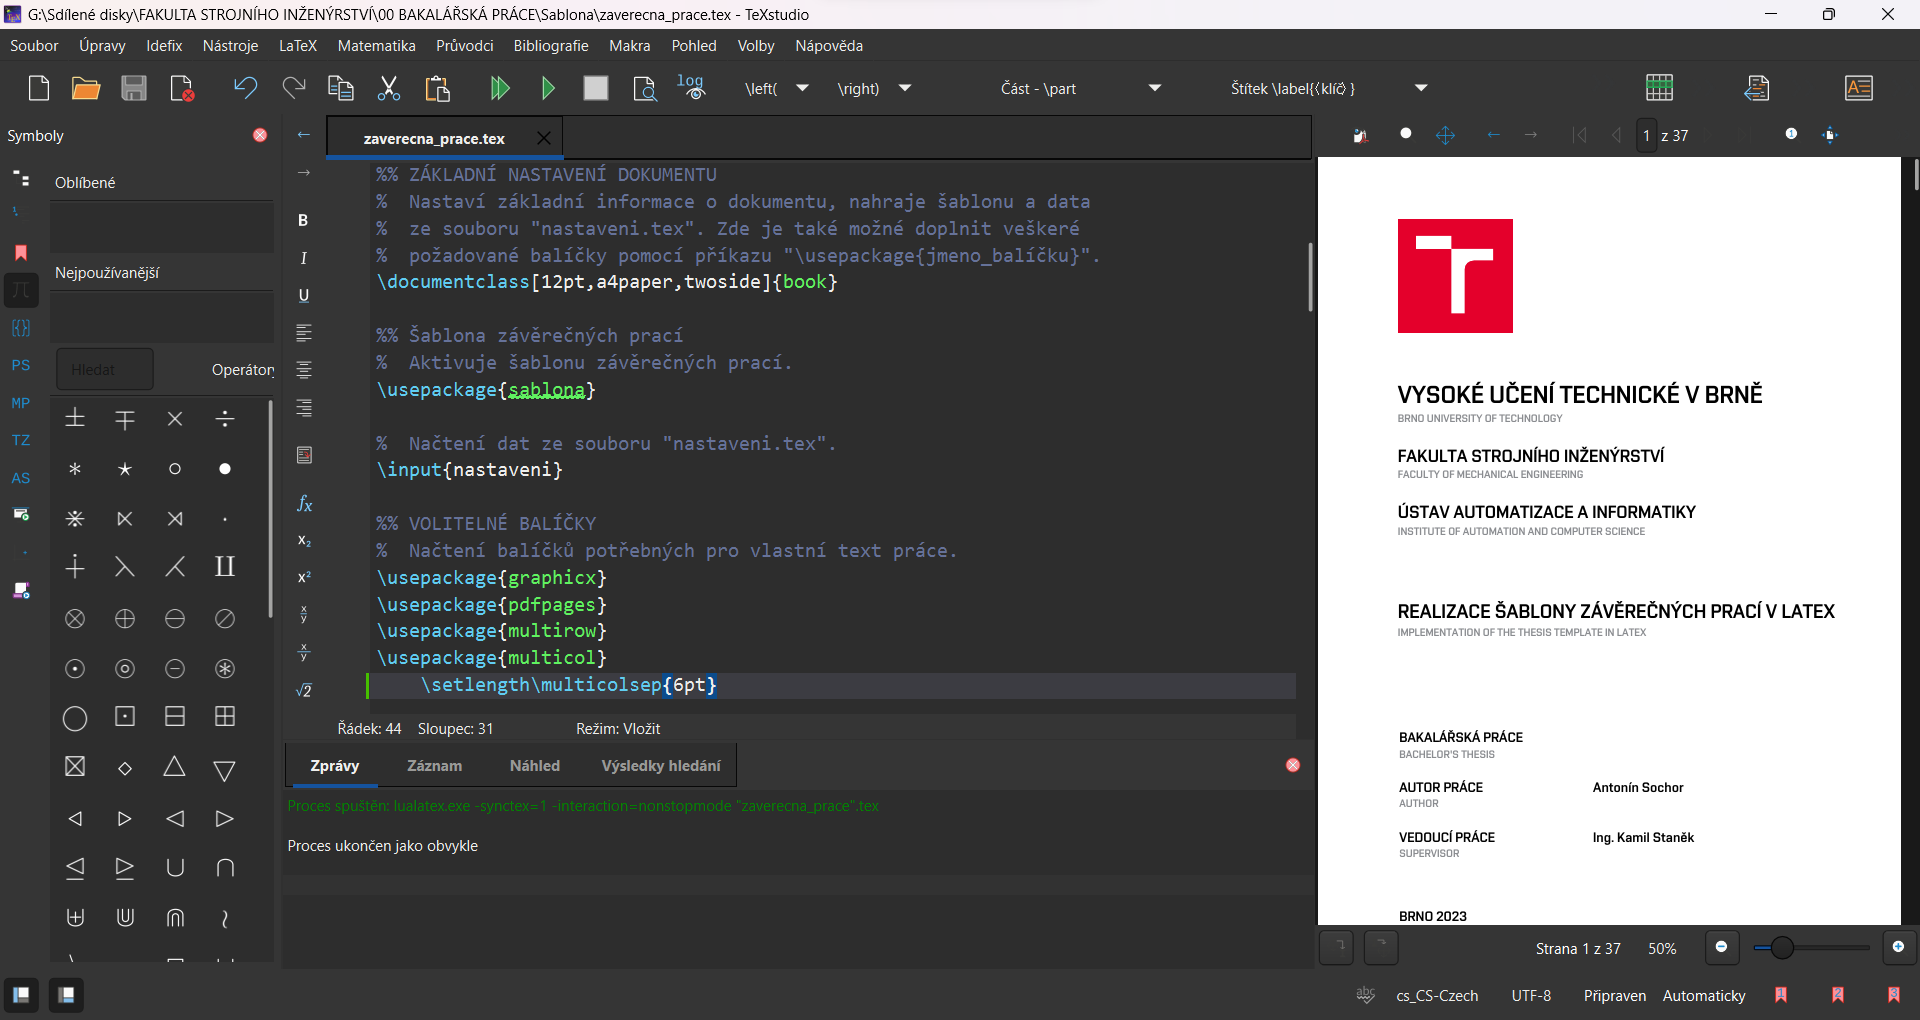
\includegraphics[width=\textwidth]{obrazky/texstudio.png}
	\caption[Ukázka prostředí \TeX studio editoru.]{Ukázka prostředí \TeX studio editoru. [vlastní]}
	\label{fig:texstudio}
\end{figure}

\TeX studio editor je dostupný na platformách Windows, Linux a macOS. Nabízí české uživatelské prostředí s kontrolou pravopisu, našeptávání \LaTeX\ příkazů, asistenta pro vkládání obrázků včetně podpory Drag \& Drop a asistenta při tvorbě tabulek. Editor má také integrovaný PDF prohlížeč překládaného dokumentu. Velkou výhodou je víceprůchodový překlad, při kterém editor automaticky spustí potřebné překladače a uživatel je tak nemusí spouštět manuálně. Editor podporuje uživatelskou volbu překladačů. Na výběr jsou \LaTeX, pdf \LaTeX, \LaTeX mk, Xe\LaTeX\ a Lua\LaTeX. \cite{Texstudiofeatures}

Nevýhodou je ve výchozím stavu nepřehledně nastavené zvýrazňování \LaTeX\ příkazů.

\textbf{Výhody a nevýhody:}
\begin{multicols}{2}
	\begin{itemize}
		\item [+] použití zdarma
		\item [+] uživatelské prostředí v českém jazyce
		\item [+] kontrola pravopisu
		\item [+] verze pro Windows, macOS i Linux
		\item [+] tlačítka pro matematické symboly
		\item [+] našeptávání příkazů
		\item [+] integrovaný PDF prohlížeč
		\item [+] automatický víceprůchodový překlad
		\item [+] asistent vkládání obrázků
		\item [+] asistent tvorby tabulek
		\item [+] podpora Drag \& Drop
	\columnbreak
		\item [--] chybějící překlad některých tlačítek
		\item [--] nevyužívá cloud
		\item [--] nepřehledné výchozí zvýrazňování
	\end{itemize}
\end{multicols}

\subsection{LyX}
Editor LyX je výkonný WYSIWYM editor. WYSIWYM je zkratkou anglické věty "What You See Is What You Mean", v češtině "Vidíš to, co máš na mysli". Jedná se tedy o editor, ve kterém uživatel zpracovává dokument podobně jako například v aplikaci Microsoft Word. Píše text, který člení na kapitoly, pomocí integrovaných nástrojů vkládá obrázky, rovnice a tabulky. Uživatel tak nevyužívá \LaTeX\ příkazy, tvoří pouze vlastní obsah. O doplnění příkazů a překlad dokumentu pomocí jazyka \TeX\ se stará editor. \cite{Lyx}

\begin{figure}[h]
	\centering
	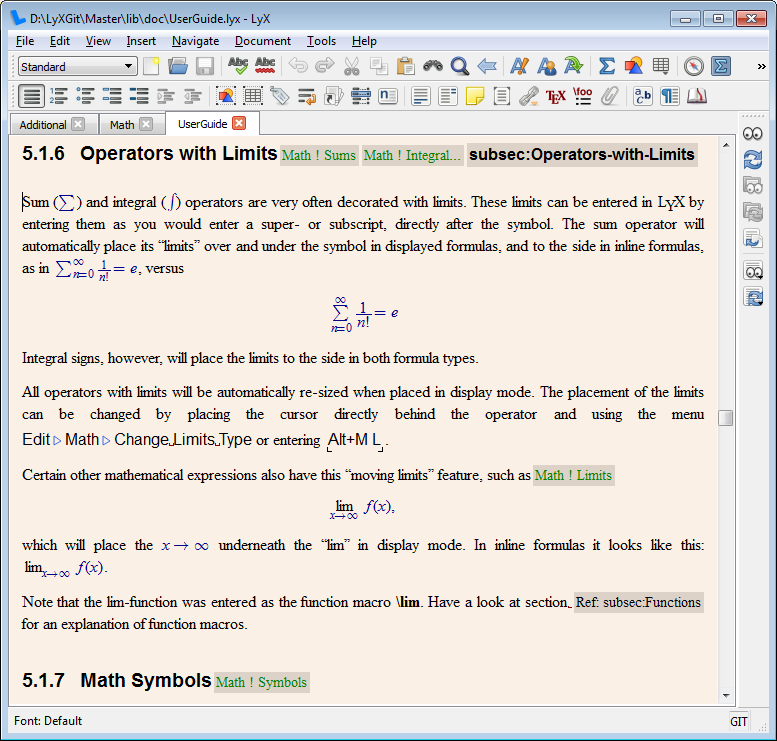
\includegraphics[width=10cm]{obrazky/lyx.png}
	\caption[Ukázka prostředí LyX editoru.]{Ukázka prostředí LyX editoru. \cite{Lyximg}}
	\label{fig:lyx}
\end{figure}

LyX je možné spustit na operačních systémech Windows, Linux i macOS. Podporuje ukládání a správu jednotlivých verzí, uživatelské prostředí je přeloženo do českého jazyka včetně podpory kontroly pravopisu. Editor má zabudovaný vlastní PDF prohlížeč tvořeného dokumentu. Autoři LyX editoru uživatelům umožňují volbu překladače. Na výběr jsou \LaTeX, pdf \LaTeX, Xe\LaTeX\ a Lua\LaTeX. \cite{Lyxfeatures}

\textbf{Výhody a nevýhody:}
\begin{multicols}{2}
	\begin{itemize}
		\item [+] použití zdarma
		\item [+] uživatelské prostředí v českém jazyce
		\item [+] kontrola pravopisu
		\item [+] verze pro Windows, macOS i Linux
		\item [+] integrovaný PDF prohlížeč
		\item [+] WYSIWYM editor
		\item [+] psaní bez \LaTeX\ příkazů
	\columnbreak
		\item [--] pracnější tvorba matematických rovnic
		\item [--] nevyužívá cloud
	\end{itemize}
\end{multicols}

\subsection{Overleaf}
Overleaf je moderní online \LaTeX\ editor, který běží na serverech poskytovatele, a uživatel tak není nucen si jej instalovat přímo do svého zařízení. K editoru se tak dostane přes libovolný webový prohlížeč. Editor se vyznačuje svou jednoduchostí a rychlostí. Nabízí registraci a používání zdarma s možností předplacení prémiové verze. Overleaf je částečně přeložen do českého jazyka, tento překlad je ale nedokonalý a neúplný -- v uživatelském prostředí jsou přeloženy pouze některé položky. Velkou výhodou je automatický víceprůchodový překlad. Overleaf také nabízí výběr z více překladačů. Integrovány jsou \LaTeX, pdf \LaTeX, Xe\LaTeX\ a Lua\LaTeX. \cite{Overleaf}

\begin{figure}[h]
	\centering
	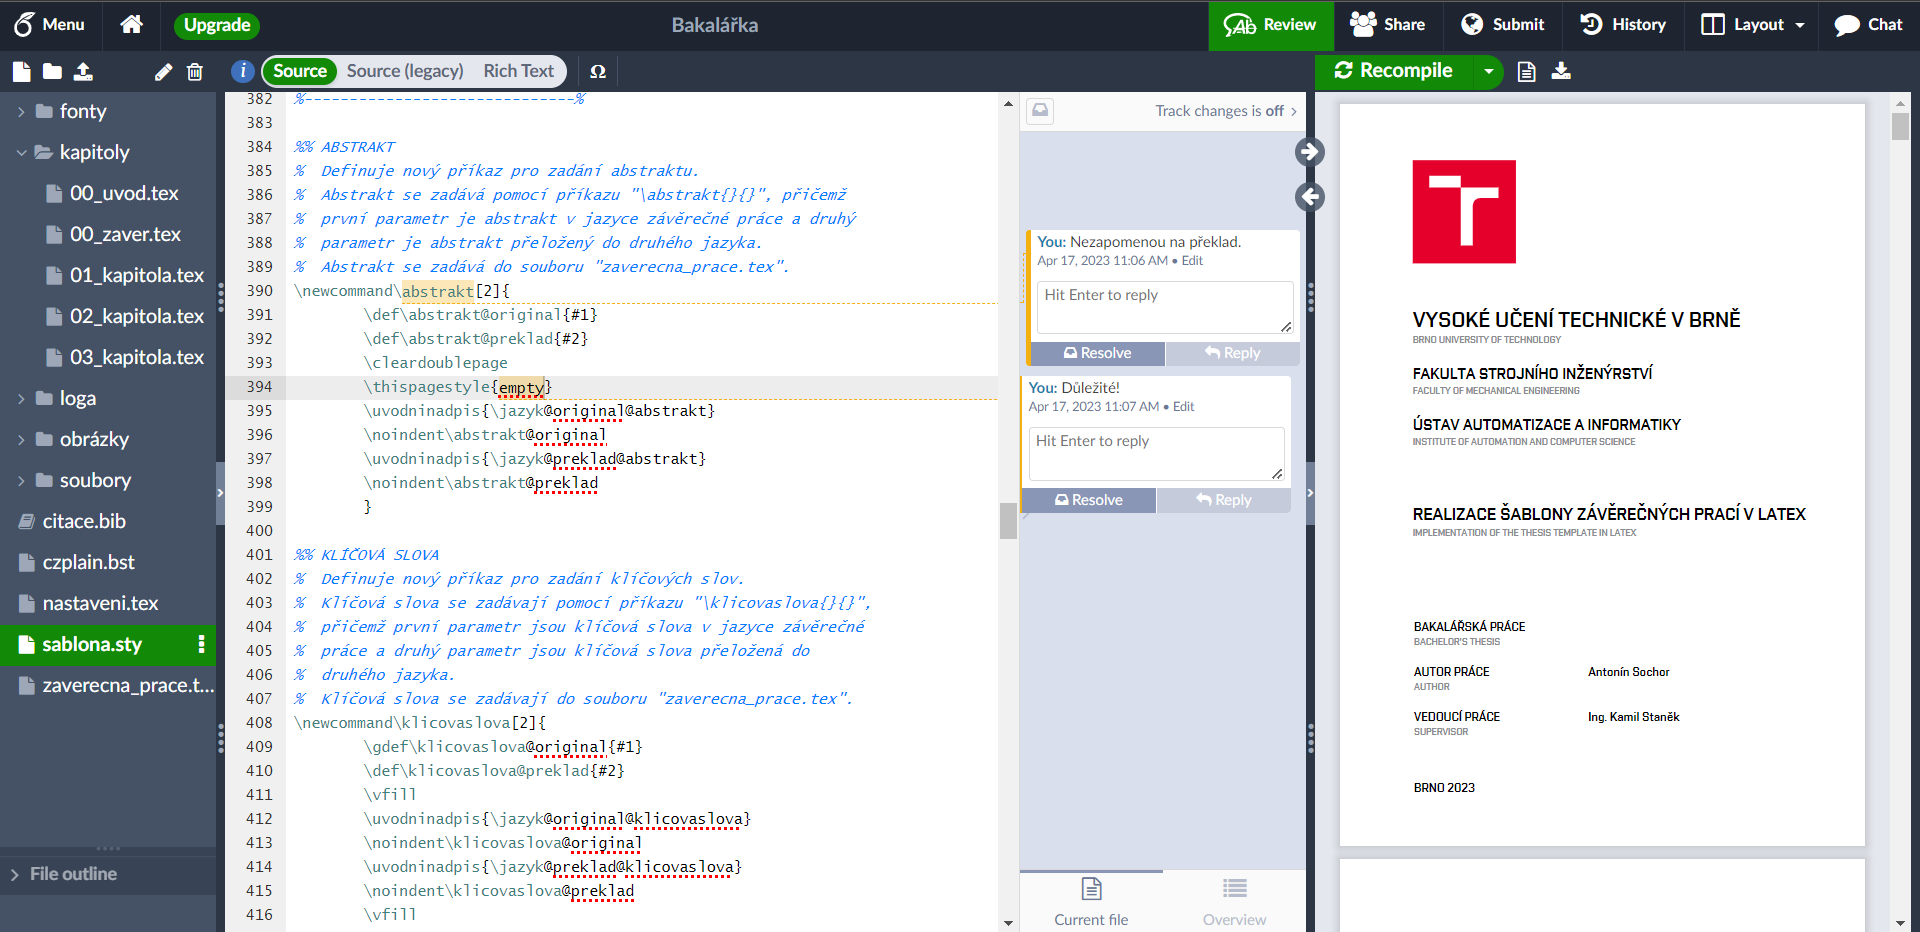
\includegraphics[width=\textwidth]{obrazky/overleaf.png}
	\caption[Ukázka prostředí Overleaf editoru.]{Ukázka prostředí Overleaf editoru. Upraveno. [vlastní]}
	\label{fig:overleaf}
\end{figure}

Neplacená verze editoru nabízí veškeré základní funkce včetně volby překladače zdrojového kódu a možnost spolupráce s jedním dalším uživatelem. Jediným omezením je časový limit pro překlad. Překladač jazyka \TeX\ má na přeložení zdrojového kódu a vygenerování výsledného dokumentu pouze jednu minutu. \cite{Overleafpremium}

Prémiová verze je rozdělena na tři balíčky, které se liší svou cenou a obsahem prémiových funkcí. K těm patří možnost spolupráce s více osobami současně, ukládání jednotlivých verzí dokumentu s možností jejich obnovení, integrace GitHubu, Dropboxu a citačních manažerů Mendeley a Zotero. Overleaf nabízí také levnější verzi předplatného pro studenty. \cite{Overleafpremiumtab}

Overleaf má nastaven limit pro počet souborů v rámci jednoho projektu. Pro každý projekt může uživatel nahrát maximálně 2000 souborů. Tento limit tak může být komplikací pro větší a náročnější projekty. \cite{Overleaflimity}

\textbf{Výhody a nevýhody:}
\begin{multicols}{2}
	\begin{itemize}
		\item [+] použití zdarma (s omezením)
		\item [+] neomezené množství projektů
		\item [+] našeptávání příkazů
		\item [+] možnost spolupráce s dalšími uživateli
		\item [+] integrovaný PDF prohlížeč
	\columnbreak
		\item [--] nedokonalý překlad do českého jazyka
		\item [--] vysoké ceny prémiových funkcí
		\item [--] omezený čas pro překlad v základní verzi
	\end{itemize}
\end{multicols}

\subsection{Papeeria}
Papeeria je online \LaTeX\ editor nabízející placenou verzi i verzi zdarma. Neplacená verze nabízí neomezené množství projektů s možností spolupráce s jinými uživateli, Git synchronizaci a možnost ukládání historie změn jednotlivých dokumentů po dobu 24 hodin. Veškeré projekty jsou veřejné, uživatel má ve verzi zdarma možnost pouze jednoho soukromého projektu. \cite{Papeeria}\cite{Papeeriafeatures}

\begin{figure}[h]
	\centering
	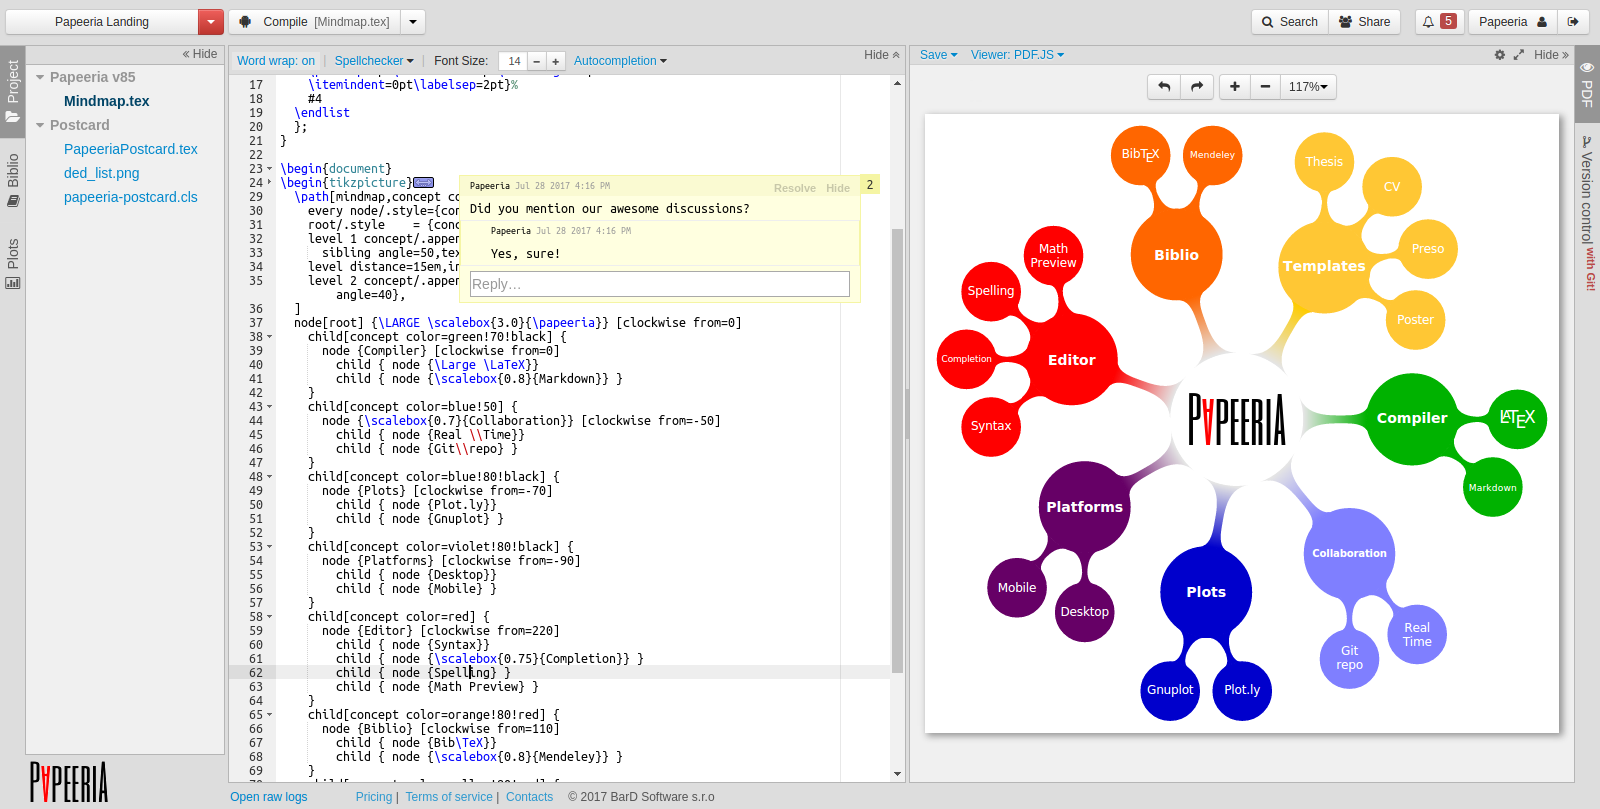
\includegraphics[width=\textwidth]{obrazky/papeeria.png}
	\caption[Ukázka prostředí Papeeria editoru.]{Ukázka prostředí Papeeria editoru. \cite{Papeeriaimg}}
	\label{fig:papeeria}
\end{figure}

Placená verze přidává možnost synchronizace s DropBoxem a Google Drivem, až deset soukromých projektů, prioritní kompilace zdrojového kódu na serveru. Uživatel má možnost obnovit historii změn dokumentů za posledních 30 dnů a také možnost využít citační manažer Mendeley. \cite{Papeeriafeatures}

Editor uživateli nabízí možnost volby překladače jazyka \TeX\ (\LaTeX, pdf \LaTeX, Xe\LaTeX\ a Lua\LaTeX) a zobrazit výsledný dokument v integrovaném PDF prohlížeči.  \cite{Papeeria}

Velkou nevýhodou Papeeria editoru je jeho zastaralost. Poslední aktualizace je z roku 2020. Nejnovější verze distribuce jazyka \TeX, kterou má uživatel možnost nastavit, je z roku 2019. Editor nenabízí českou lokaci. \cite{Papeeria}

\textbf{Výhody a nevýhody:}
\begin{multicols}{2}
	\begin{itemize}
		\item [+] použití zdarma (s omezením)
		\item [+] neomezené množství projektů
		\item [+] našeptávání příkazů
		\item [+] možnost spolupráce s dalšími uživateli
		\item [+] integrovaný PDF prohlížeč
		\item [+] možnost předplatného
		\item [+] ukládání historie změn
	\columnbreak
		\item [--] pouze jeden soukromý projekt.
		\item [--] absence překladu prostředí do českého jazyka
		\item [--] zastaralá verze jazyka \TeX
		\item [--] poslední aktualizace v roce 2020
		\item [--] problémové nahrávání souborů
	\end{itemize}
\end{multicols}

%--------------------------------------------------%
